
\hspace{20 px} Since Bernhard Riemann, mathematician knew that only a finite number of parameters can describe a geometric hyperbolic surface. Considering this, we can be interested in the set of all geometry we can give to a given surface, modulo composition by map isotopic the identity, this set is called the Teichmuller space. Moreover other problem rise shortly after this definition. How can we deform in the natural way a geometry of a surface into an other? What does it mean that two geometries are closed one to each other? What are the natural boundaries of the Teichmuller space?

\begin{wrapfigure}{r}{5cm}[!ht]
  \centering
  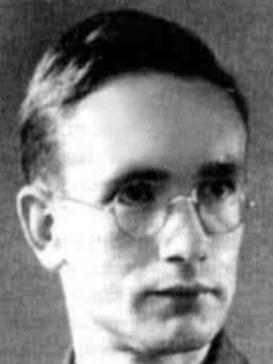
\includegraphics[width=4cm]{Image/Teichmuller.jpeg}
  \caption{The mathematician Oswald Teichmuller}
\end{wrapfigure}

\vspace{10 px}

Oswald Teichmuller, a german mathematician, gave answers to this question in the year preceding the second World war.He create the first metric on this space by finding a solution to an extremal problem: between two hyperbolic geometry on the same surface is there a function which minimize the deformation. the theorem not only prove the existence, but also the unicity of this function. It naturraly create a distance in the now called Teichmuller space by considering the logarithm of the deformation of the extremal function.

\vspace{10 px}

Thurston then added other important steps to this theory. He underligned the role of laminations which are a generalisation of simple closed curve. And he created the earthquake flow which turn to play an important role in Teichmuller theory.
Kerckhoff used this tool to show the Nielsen realisation conjecture in 1983 \cite{NielsenRealizationPro} which state that every finite subgroup of the mapping class group have a fixed point in the Teichmuller space.

This theory have generated a lot of litterature and now some book are classic introduction to this subject. We can cite \cite{farb2011primer}, \cite{hubbardhal01297628}, \cite{kapovich2009hyperbolic} or the course notes \cite{Mcmullen1998HyperbolicM} and \cite{Mcmullen1998Riemann}.

\vspace{10 px}

An important question in Hyperbolic geometry is the asymptotic number of closed geodesic. To begin we can ask the number $\pi(X,L)$ of closed geodesic on a hyperbolic surface of length less than $L$. The answer was found by Delsarte, Huber and Selberg \cite{buser2010geometry}
 and is called the prime number theorem for hyperbolic surfaces (because of the ressemblance to the prime number theorem). It states that \[
\pi(X,L) \equiv e^{L} / L
\]
as $L \to \infty$.
A much harder question was to find the number, $\sigma(X,L)$, of simple (which don't intersect themselves) closed geodesic of length less than $L$ on a hyperbolic surface $X$. It was found years later, in Mirzakhani's PhD, and we have \[
\sigma(X,L) \equiv C_{X}L^{6g-6}
\]
As $L \to \infty$ where $g$ is the genus of the surface $X$ and $C_{X}$ is a constant which depent of the geometry $X$.
To do that Myriam Mirzhakhani conjugated the earthquake flow to the horocycle flow. This step give that the Earthquake flow is ergodic and allow us to use Birkoff theorem to understand asymptotic quantities.

\vspace{10 px}

The question is now to give error term to this quantity and to do that we need to understand better the mixing rate of the earthquake flow. This flow is conjugate to the horocyclic flow which has a polynomial mixing rate. But as the conjugacy is only a measurable map it does not transport the rate of mixing. We should analyse the rate of mixing of the earthquake flow by other means. One is to consider natural functions on Teichmuller space such as the systole which is the lenth of the shortest simple closed curve on the surface. This function behave nicely along earthquake path, it is continuous, convex and we know the first derivative at the origin. Moreover in the case of the once ponctured torus we can
give a frame determined by the continued fraction of the slope.

\vspace{10 px}

In this master thesis, I will first give an introduction to Teichmuller theory and some useful and classic tools in this theory such as the collar lemma or the decomposition of a surface in pair of pant. Then we will review the proof of the Mirzhakani conjugacie between the horocyclic flow and the earthquake flow. We will after talk about the mixing proprities of the ergofic and horocyclic flow, and discuss theirs mixing rate. Finally we will discuss of a special case which can be the most simple example of hyperbolic surface, that is the once ponctured torus.
